\section{Shingeki no Kyojin - C3 2013-1}

Hace cientos de años, los humanos fueron casi masacrados por Titanes, seres no inteligentes que devoran humanos. La sociedad se ha guarecido en ciudades protegidas por grandes murallas y donde la única forma de contraatacar es a través del escuadrón de reconocimiento. Para mantener un orden, este escuadrón mantiene un registro de todos sus miembros en un archivo con la estructura \texttt{nombre:edad:genero:ranking, rango,habilidad}, como en el siguiente archivo de ejemplo

\begin{figure}[h]
    \centering
    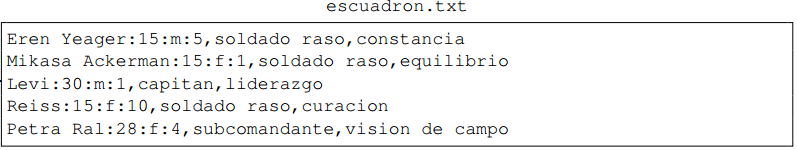
\includegraphics[scale=0.8]{Imagenes/escuadron.png}
\end{figure}

Tras salir a combatir existen muchas bajas, por eso necesitan mantener un registro actualizado constantemente. Para ello:

\begin{itemize}
    \item[a)] Desarrolle una función \texttt{listar\_bajas(rango, registro, bajas)}, la cual recibe el \texttt{rango} de los soldados a listar, un string \texttt{registro} que especifica el nombre del archivo con los soldados y una lista de \textbf{True} y \textbf{False}, siendo \textbf{True} si el soldado aún vive o \textbf{False} si no. La función retorna una lista con tuplas con el nombre, edad, género y ranking de los soldados muertos (bajas) en el rango especificado.
    
    \begin{lstlisting}[style=consola]
>>> listar_bajas("soldado raso", "escuadron.txt", [False,True,False])
[('Eren Yeager', '15', 'm', '5'), ('Reiss', '15', 'f', '10')]
    \end{lstlisting}
    \item[b)] Desarrolle una función \texttt{promedio\_edad(bajas)}, la cual recibe la lista \texttt{bajas} (como la generada en la pregunta a) ) y retorna el promedio de edad de los soldados en dicha lista. Redondee el promedio
    
    \begin{lstlisting}[style=consola]
>>> bajas=listar_bajas("soldado raso", "escuadron.txt", [False,True,False])
>>> promedio_edad(bajas)
15.0
    \end{lstlisting}
    \item[c)] Cree la función \texttt{actualizar\_registro(registro, bajas)}, la cual recibe como parámetro un string correspondiente al nombre del archivo con los datos de las tropas(\texttt{registro}) y una lista de tuplas con los datos de los soldados de bajas (\texttt{bajas}). Esta función debe crear un nuevo archivo, llamado \texttt{nuevo\_ + nombre\_del\_archivo}, ver ejemplo. Este archivo debe contener sólo los soldados sobrevivientes. La función no tiene retorno.
    
    \begin{lstlisting}[style=consola]
>>> actualizar_registro('escuadron.txt',bajas)
>>> 
    \end{lstlisting}
    
    \begin{figure}[h]
        \centering
        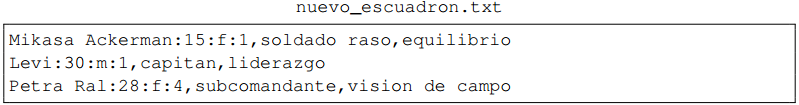
\includegraphics[scale=0.8]{Imagenes/nuevoescuadron.png}
    \end{figure}
\end{itemize}